\section{Edge Detection}

\subsection{What is an Edge?}
\marginpar{\kaishu Step 1: 问题定义, problem formulation.}
“边缘”是图像中的一个区域,在这个区域中,沿着图像的一个方向,
像素强度值 (或者说对比度) 发生了“显著(Significant)”的变化,而在其正交方向上,
像素强度值 (或对比度) 几乎没有变化.

注意: Gradient magnitude 大的地方不一定是边缘, 可能是多个方向差分都有显著变化, 即边缘交叉处或者可能是噪声.

\subsection{Criteria for Optimal Edge Detection}
\marginpar{\kaishu Step 2: 评价标准, evaluation metrics.}
我们使用 Accuract, Precision, Recall 来评价边缘检测的好坏.
\[
\begin{array}{c|cc}
    \hline
     & \text{Postive} & \text{Negative} \\
    \hline
    \text{True} & \text{True Positive (TP)} & \text{False Negative (FN)} \\
    \text{False} & \text{False Positive (FP)} & \text{True Negative (TN)} \\
    \hline
\end{array}
\]

具体定义如下:
\begin{equation}
\text{Accuracy}=\frac{\text{TP}+\text{TN}}{\text{TP}+\text{FP}+\text{TN}+\text{FN}} 
\end{equation}

\begin{equation}
\text{Precision}=\frac{\text{TP}}{\text{TP}+\text{FP}} 
\end{equation}

\begin{equation}
\text{Recall}=\frac{\text{TP}}{\text{TP}+\text{FN}}
\end{equation}

Precision 和 Recall 都代表着你检测出的真正边缘所占比例,但是 Precision 的分母
是你检测出的边缘,Recall 的分母是真正的边缘.好的边缘检测算法应满足:
\begin{itemize}
    \item High precision: 确保所有检测到的边都是正确的 (via minimizing FP).
    \item High recall: 确保所有边都被检测到 (via minimizing FN).
    \item Good localization: 边缘检测的边缘应该尽可能的靠近真实边缘.
    \item Single response constraint: 最小化响应的数量.
\end{itemize}

在后续物体检测任务中会定义Precision-Recall Curve 和 Average Precision, 以综合考虑 Precision 和 Recall.

\subsection{Smoothing by Gaussian Filter}
由于上述提及的 Gradient magnitude 在每个像素点的值都非零, 且梯度对于噪声敏感, 难以从中直接将
边缘提取出来, 所以我们需要对图像进行平滑处理. 

这里我们使用 Gaussian Filter, 它是一个低通滤波器, 且Gaussian kernel的傅立叶变换是一个还是一个 Gaussian kernel, 即
\[
    g = \frac{1}{\sqrt{2\pi}\sigma} \exp\left( -\frac{x^2}{2\sigma^2} \right), \quad \mathcal{F}(g) = \exp \left( -\frac{\sigma^2\omega^2}{2} \right)
\]
\begin{itemize}
    \item 当 $\sigma$ 越大时, $\mathcal{F}(g)$ 越集中于低频, 当 $\sigma \to \infty$ 时, 会滤过所有高频只留下常数信号.
    \item 当 $\sigma$ 越小时, $\mathcal{F}(g)$ 越分散, 会保留更多高频信号.
\end{itemize}
在实际运算中会用到一个小技巧来减少计算量, Derivative Theorem of Convolution:
\[
\frac{\dd }{\dd x} (f * g) = f * \frac{\dd }{\dd x} g
\]
那么可以将运算从两步(先求导, 再卷积)变为一步(直接卷积).


\subsection{Non-Maximal Suppression (NMS)}

非最大值抑制,顾名思义,就是抑制非最大值,这里的最大值指的是梯度的局部最大值.

在计算出了所有点的梯度之后,会有很多像素的梯度大于设定的阈值,而我们希望最后得出的边缘像素真的看起来
像一条线而不是一块区域,所以 NMS 的目的是为了抑制那些不是边缘的像素,只保留那些是边缘的像素.

\begin{figure}[htbp]
    \centering
	\includegraphics[scale=0.2]{figures/NMS.png}
	\caption{NMS示意图}
\end{figure}

对于一个边缘像素的候选点,我们认为它是边缘当:它比它梯度方向的两个点 $q+\nabla q$ 和 $q-\nabla q$ 的梯度值大,
也就是这个点的梯度大小是局部最大值的时候.

\begin{figure}[htbp]
    \centering
	\includegraphics[scale=0.4]{figures/bilinear.png}
	\caption{双线性插值}
\end{figure}

计算这个点梯度方向的点的梯度值可以使用双线性插值法,就是把这个点周围的四个点的梯度按照横纵距离反比加权.

当然,NMS 是一个思想而不是针对边缘检测的算法,比如对于 keypoint detection,object detection (like YOLO) 都可以使用 NMS,
实现的思路都很类似,使用一个打分函数看这个备选点 (bounding box) 是不是比跟它相邻 (冲突) 的点 (bounding box) 好,如果是就保留,否则就抑制.

\subsection{A Simplified Version of NMS}

\begin{figure}[htbp]
    \centering
	\includegraphics[scale=0.55]{figures/simple_NMS.png}
	\caption{简化版本的双线性插值}
\end{figure}

一个 NMS 的简化版本是把双线性插值省去,直接让这个像素的梯度大于它梯度方向的那两个相邻像素的梯度.

\subsection{Edge Linking: Hysteresis Thresholding}
遍历每个像素点, 使用高阈值 (maxVal) 开始边缘曲线,使用低阈值 (minVal) 继续它们.

\begin{itemize}
    \item Pixels with gradient magnitudes > maxVal should be reserved.
    \item Pixels with gradient magnitudes < minVal should be removed.
\end{itemize}

How to decide maxVal and minVal? Examples:

\begin{itemize}
    \item maxVal = 0.3 $\times$ average magnitude of the pixels that pass NMS
    \item minVal = 0.1 $\times$ average magnitude of the pixels that pass NMS
\end{itemize}
\begin{figure}[htbp]
    \centering
    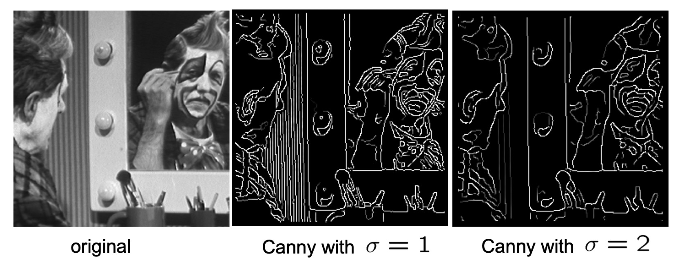
\includegraphics[scale=0.4]{figures/canny.png}
    \caption{Canny Edge Detection with Different $\sigma$}
\end{figure}
上述过程就是经典的 Canny Edge Detection 算法, 算法的核心是使用了 Gaussian Filter, 超参数为 $\sigma$, $\sigma$ 越大时, 越会关注更显著的边缘.
